\documentclass[conference]{IEEEtran}
\IEEEoverridecommandlockouts
% The preceding line is only needed to identify funding in the first footnote. If that is unneeded, please comment it out.
\usepackage{cite}
\usepackage{amsmath,amssymb,amsfonts}
\usepackage{algorithmic}
\usepackage{graphicx}
\usepackage{textcomp}
\usepackage{xcolor}
\def\BibTeX{{\rm B\kern-.05em{\sc i\kern-.025em b}\kern-.08em
    T\kern-.1667em\lower.7ex\hbox{E}\kern-.125emX}}
\begin{document}

\title{Performace on differnet parameter setting in GA-BPNN\\
% {\footnotesize \textsuperscript{*}Note: Sub-titles are not captured in Xplore and should not be used}
% \thanks{Identify applicable funding agency here. If none, delete this.}
}

% \author{\IEEEauthorblockN{1\textsuperscript{st} Given Name Surname}
% \IEEEauthorblockA{\textit{dept. name of organization (of Aff.)} \\
% \textit{name of organization (of Aff.)}\\
% City, Country \\
% email address or ORCID}
% \and
% \IEEEauthorblockN{2\textsuperscript{nd} Given Name Surname}
% \IEEEauthorblockA{\textit{dept. name of organization (of Aff.)} \\
% \textit{name of organization (of Aff.)}\\
% City, Country \\
% email address or ORCID}
% \and
% \IEEEauthorblockN{3\textsuperscript{rd} Given Name Surname}
% \IEEEauthorblockA{\textit{dept. name of organization (of Aff.)} \\
% \textit{name of organization (of Aff.)}\\
% City, Country \\
% email address or ORCID}
% \and
% \IEEEauthorblockN{4\textsuperscript{th} Given Name Surname}
% \IEEEauthorblockA{\textit{dept. name of organization (of Aff.)} \\
% \textit{name of organization (of Aff.)}\\
% City, Country \\
% email address or ORCID}
% \and
% \IEEEauthorblockN{5\textsuperscript{th} Given Name Surname}
% \IEEEauthorblockA{\textit{dept. name of organization (of Aff.)} \\
% \textit{name of organization (of Aff.)}\\
% City, Country \\
% email address or ORCID}
% \and
% \IEEEauthorblockN{6\textsuperscript{th} Given Name Surname}
% \IEEEauthorblockA{\textit{dept. name of organization (of Aff.)} \\
% \textit{name of organization (of Aff.)}\\
% City, Country \\
% email address or ORCID}
% }

\maketitle

\begin{abstract}
GA-BANN is an easy and well-known hybrid network. However, it's difficult to finds to goood solution beacause the paramerters of backpropagation neutral network is large. This paper want to discuss the differnet strategies to run GA-BPNN, and test which performace is better. 
\end{abstract}

\begin{IEEEkeywords}
GA-BPNN, genetic algorithm, backpropagation
\end{IEEEkeywords}

\section{Introduction}
GA-BANN is a two-layers hybrid network. First uses genetic algorithm to evolute paramerters, then apply to backpropagation. It is to implement. However, due to the range of paremeters is infinity. The accuracy rate of GA-BPNN is often low. To solve this, we revise the genetic algorithm part to improve accuracy rate.\\

Genetic algorithm involves population, crossover, mutation. Backpropagation neutral network involves weight, bias, the number of neurons in hidden layer and dropout. The genetic algorithm will adjust weight and bias.\\ 

\subsection{Genetic algorithm}
Genetic algorithm is a method inspired by the natural process. The process can be divide into 6 parts.\\

First is generating population the process will generate $L$ population.\\

Second part is evaluate the every poppulation's fitness, the fitness can be defined widely. In GA-BPNN, we can defined the the accuracy rate of testing data.\\

Third is parent selection, we use 2-tournament selection, that is, select 2 parents randomly and retain the one has higher fitness.\\

The fourth step is crossover. We define a constant, $p_c$, is the rate of crossover, and use random function as roulette. When the result of roulette is $< p_c$ do crossover, otherwise not to do.\\

After crossover is mutation, like crossover, $p_m$ is the 
rate of mutation.\\

Final is surival selection, select best $L$ population from parents or offspring based on fitness. That's the whole process of genetic algorithm.\cite{b1}\\

\begin{figure}[htbp]
\centerline{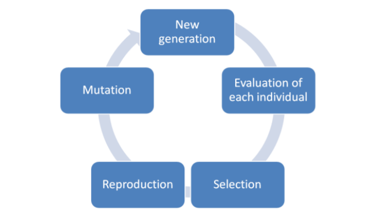
\includegraphics{Genetic_algorithm.png}}
\caption{Process of Genetic Algorithm}
\label{fig}
\end{figure}

\subsection{Backpropagation Neutral Network}
Backpropagation Neutral Network is a three-layers neutral network. Fisrt is input layer, second is hidden layer, third is output layer.\cite{b2}\\

\begin{figure}[htbp]
\centerline{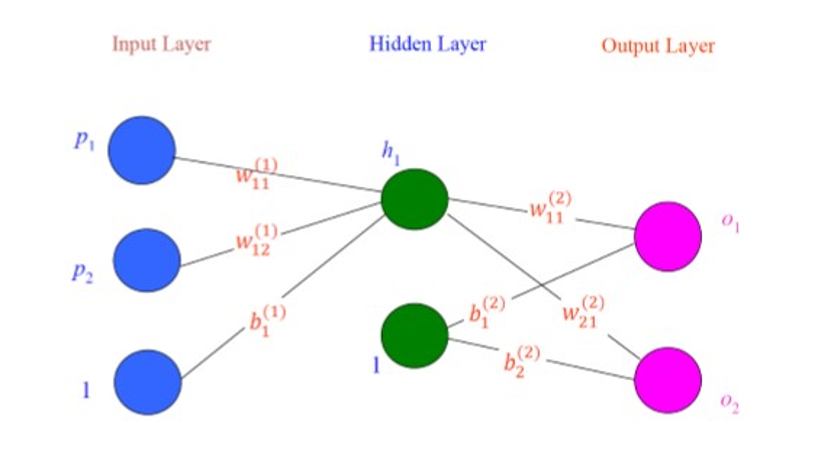
\includegraphics[width=10cm]{Backpropagation.png}}
\caption{Backpropagation Structure}
\label{fig}
\end{figure}

It uses gradient descent to adjust weight and bias.\\

\begin{equation}
\label{gradient_descent}
\nabla f(x, y) = \left[
\begin{array}{ccc}
\frac{\partial f(x, y)}{\partial x}\\
\frac{\partial f(x, y)}{\partial y}\\
\end{array}
\right]
\end{equation}

\begin{thebibliography}{00}
\bibitem{b1} Li Jiacheng and Li Lei
, A Hybrid Genetic Algorithm Based on Information Entropy and Game Theory, IEEEAccess Volume 8, 2020
\bibitem{b2} Martin T. Hagan Oklahoma State University Stillwater, Oklahoma Howard B. Demuth University of Colorado Boulder, Colorado Mark Hudson Beale MHB Inc. Hayden, Idaho Orlando De Jesús Consultant Frisco, Texas, Neural Network Design 2nd Edtion 

\end{thebibliography}
\vspace{12pt}

\end{document}
